\documentclass{article}
\PassOptionsToPackage{numbers,compress}{natbib}
\usepackage[final]{neurips}
\usepackage[utf8]{inputenc}
\usepackage[T1]{fontenc}
\usepackage{hyperref}
\usepackage{url}
\usepackage{booktabs}
\usepackage{amsfonts}
\usepackage{amsmath}
\usepackage{nicefrac}
\usepackage{microtype}
\usepackage{xcolor}
\usepackage{graphicx}

\title{VAE vs. DDPM for Image Generation on Fashion-MNIST}

\author{%
  Yuye Huang\\
  Department of Electrical and Computer Engineering\\
  University of Toronto\\
  \texttt{yuye.huang@mail.utoronto.ca} \\
  % more authors
  \And
  Jenny You\\
  Department of Mechanical and Industrial Engineering\\
  University of Toronto\\
  \texttt{Jenny.You@mail.utoronto.ca} \\
  \And
  Jasmine Shao\\
  Department of Mechanical and Industrial Engineering\\
  University of Toronto\\
  \texttt{jasmine.shao@mail.utoronto.ca} \\
}

\begin{document}
\maketitle

\begin{abstract}
This project compares a convolutional Variational Autoencoder (VAE) and a Denoising Diffusion Probabilistic Model (DDPM) for image generation on Fashion-MNIST. Both models were trained on the same dataset and evaluated with a shared pipeline using generated image samples, classifier-based feature metrics, class-distribution statistics, and measured computational cost. The DDPM produced sharper and more recognizable samples and achieved substantially lower classifier-feature FID and KID than the VAE. It also generated a more balanced class distribution. In contrast, the VAE required much less training time and generated samples almost immediately through a single decoder pass. The results show a clear trade-off between generation quality and computational efficiency for the two generative approaches.
\end{abstract}

\section*{Statement of Team Contributions}
All group members contributed to problem framing, implementation planning, experimental design, result interpretation, and final review. Jenny primarily worked on the VAE implementation, training pipeline, and latent-space experiments. Yuye primarily worked on the DDPM implementation, diffusion training and sampling pipeline, and denoising visualizations. Jasmine primarily handled the shared evaluation pipeline, quantitative metric analysis, result comparison, and report integration.

\section{Introduction}
Generative models learn patterns from observed data and use them to create new samples. In this project, we compare two generative approaches covered in the course: Variational Autoencoders (VAEs) and Denoising Diffusion Probabilistic Models (DDPMs). A VAE represents an image through a lower-dimensional latent variable and generates new images by sampling and decoding from this latent space [1]. A DDPM instead starts from Gaussian noise and generates an image through a sequence of learned denoising steps [2].

The goal of this project is to compare these two approaches under the same Fashion-MNIST experimental setting. Fashion-MNIST contains 60,000 training images and 10,000 test images of 28$\times$28 grayscale clothing items from 10 classes [3]. Rather than selecting a single ``best'' model, we focus on their practical trade-offs. We compare generated sample quality, distribution similarity, class diversity, generation behavior, training stability, and computational cost. This allows us to study both how the two models generate images and what is gained or lost when using a more computationally expensive diffusion process. Our central research question is therefore: \emph{how much distributional and perceptual improvement does iterative diffusion provide over direct latent-variable decoding, and what training, memory, and sampling costs accompany that improvement?}

\section{Preliminaries and Problem Formulation}
Let $x \sim p_{\mathrm{data}}(x)$ denote an image from the Fashion-MNIST data distribution. The general objective is to train a generative model that can produce new samples with a distribution close to $p_{\mathrm{data}}$. We implement one VAE and one DDPM and evaluate both with the same real-image reference set and the same downstream evaluation tools.

For the VAE, the encoder estimates a Gaussian posterior $q_\phi(z\mid x)$ with mean $\mu$ and log variance $\log\sigma^2$. A latent variable is sampled using the reparameterization trick, $z=\mu+\sigma\epsilon$, where $\epsilon\sim\mathcal{N}(0,I)$, and the decoder models $p_\theta(x\mid z)$. Training minimizes a reconstruction term together with the KL divergence between the approximate posterior and the standard Gaussian prior.

More explicitly, the evidence lower bound balances two competing goals. The reconstruction term encourages preservation of image-specific detail, while the KL term regularizes the aggregate latent representation toward a sampleable prior. Strong regularization improves latent-space continuity but can sacrifice high-frequency detail, which provides one explanation for the characteristic smoothness of VAE outputs.

For the DDPM, a forward diffusion process gradually adds Gaussian noise to a clean image. At timestep $t$, the noisy sample can be written as
\begin{equation}
 x_t=\sqrt{\bar{\alpha}_t}x_0+\sqrt{1-\bar{\alpha}_t}\epsilon,
 \qquad \epsilon\sim\mathcal{N}(0,I).
\end{equation}
The neural network is trained to predict the added noise from $x_t$ and $t$. During generation, the model begins from random Gaussian noise and repeatedly applies the learned reverse denoising process until an image is produced.

Unlike the VAE bottleneck, the DDPM objective does not require a single low-dimensional code to preserve the whole image. The model instead learns local denoising decisions across multiple noise levels. This repeated refinement can recover sharper structure, but sampling cost grows approximately linearly with the number of reverse steps because those network evaluations are sequential.

\section{Design}
The project uses one shared data and evaluation pipeline for both models. Fashion-MNIST is loaded through Torchvision. The VAE is trained directly on images in the range $[0,1]$, while DDPM inputs are mapped to $[-1,1]$ before the forward noising process and mapped back to $[0,1]$ after sampling. After training, each model generates 5,000 images for evaluation.

A separate Fashion-MNIST CNN classifier is trained only for evaluation in each run. Across ten seeds it reaches $91.37\% \pm 0.20\%$ test accuracy and provides both class probabilities and 128-dimensional intermediate feature vectors. These outputs are used to measure generated-image recognizability, class distribution, classifier-feature FID/KID, and nearest-neighbor distances. This classifier is not part of either generative model. Using the same evaluator design gives both models a common comparison setting within every seed.

\section{Methodology}
\textbf{VAE.} The VAE uses a convolutional encoder with two stride-2 convolution layers, followed by a fully connected layer that outputs a 32-dimensional latent mean and log variance. After reparameterization, the decoder uses fully connected layers and two transposed convolutions to recover a 28$\times$28 image. The loss is
\begin{equation}
 \mathcal{L}_{\mathrm{VAE}}=\mathcal{L}_{\mathrm{BCE}}+\beta D_{\mathrm{KL}}(q_\phi(z\mid x)\|p(z)),
\end{equation}
with $\beta=1$. The model is trained with AdamW, cosine learning-rate decay, and gradient clipping.

\textbf{DDPM.} The DDPM uses 100 diffusion steps with a cosine noise schedule. Its noise-prediction network is a small U-Net with residual time-conditioned blocks, skip connections, sinusoidal timestep embeddings, and a self-attention block at the bottleneck. At every training iteration, a random timestep is selected, Gaussian noise is added to the input, and the network predicts that noise. The objective is mean squared error between the predicted and true noise. An exponential moving average (EMA) of the model parameters with decay 0.995 is used for final sampling. The DDPM is also trained with AdamW, cosine learning-rate decay, and gradient clipping.

\textbf{Evaluation.} Distribution similarity is measured using FID [4] and KID [5], but with 128-dimensional features from our Fashion-MNIST classifier rather than ImageNet Inception features. We therefore report them as \emph{classifier-feature FID} and \emph{classifier-feature KID}; the values should not be compared directly with standard Inception-based scores from other papers. We also measure classifier confidence, the proportion of generated samples with confidence at least 0.8, class coverage, normalized class-distribution entropy, Sobel edge sharpness, nearest-neighbor distance, training time, sampling time, trainable parameter count, and peak GPU memory.

Classifier-feature FID compares Gaussian approximations to the real and generated feature distributions through their means and covariances. Lower values indicate closer first- and second-order feature statistics. KID estimates squared maximum mean discrepancy using a polynomial kernel and does not require the same Gaussian assumption. Reporting both reduces dependence on one distributional summary. Normalized class entropy is computed from the evaluator's predicted class proportions and equals one for a uniform distribution across all ten classes. These automated measures are interpreted jointly with sample grids because evaluator confidence can reward recognizable prototypes without fully measuring visual realism or intra-class variation.

\section{Numerical Experiments}
\subsection{Experimental Setup}
The report-profile experiment uses the full 60,000-image Fashion-MNIST training set and 10,000-image test set and is repeated independently for random seeds 0 through 9. Each seed trains a new evaluator, VAE, DDPM, and EMA model and generates 5,000 samples per generator, giving 50,000 generated evaluation samples per model across the study. Training and evaluation were run in PyTorch 2.11.0 with CUDA 12.8 on an NVIDIA GeForce RTX 5070 Ti. Table~\ref{tab:config} summarizes the main model settings. The VAE is trained for 25 epochs and the DDPM for 35 epochs. Both use a batch size of 1024. Unless otherwise stated, numerical results report the mean and sample standard deviation across ten seeds.

\begin{table}[t]
\caption{Main experimental configuration.}
\label{tab:config}
\centering
\small
\begin{tabular}{lcc}
\toprule
Setting & VAE & DDPM \\
\midrule
Epochs & 25 & 35 \\
Batch size & 1024 & 1024 \\
Learning rate & $2\times10^{-3}$ & $2\times10^{-4}$ \\
Latent dimension / diffusion steps & 32 & 100 \\
Trainable parameters & 1.70M & 5.22M \\
\bottomrule
\end{tabular}
\end{table}

\subsection{Qualitative Comparison}
Figure~\ref{fig:samples} compares real Fashion-MNIST samples with samples generated by both models. Both models learn recognizable clothing shapes, but the VAE samples are generally blurrier and some outlines are less distinct. The DDPM samples have clearer edges and more recognizable object structure. This visual difference is consistent with the quantitative results reported below.

\begin{figure}[t]
  \centering
  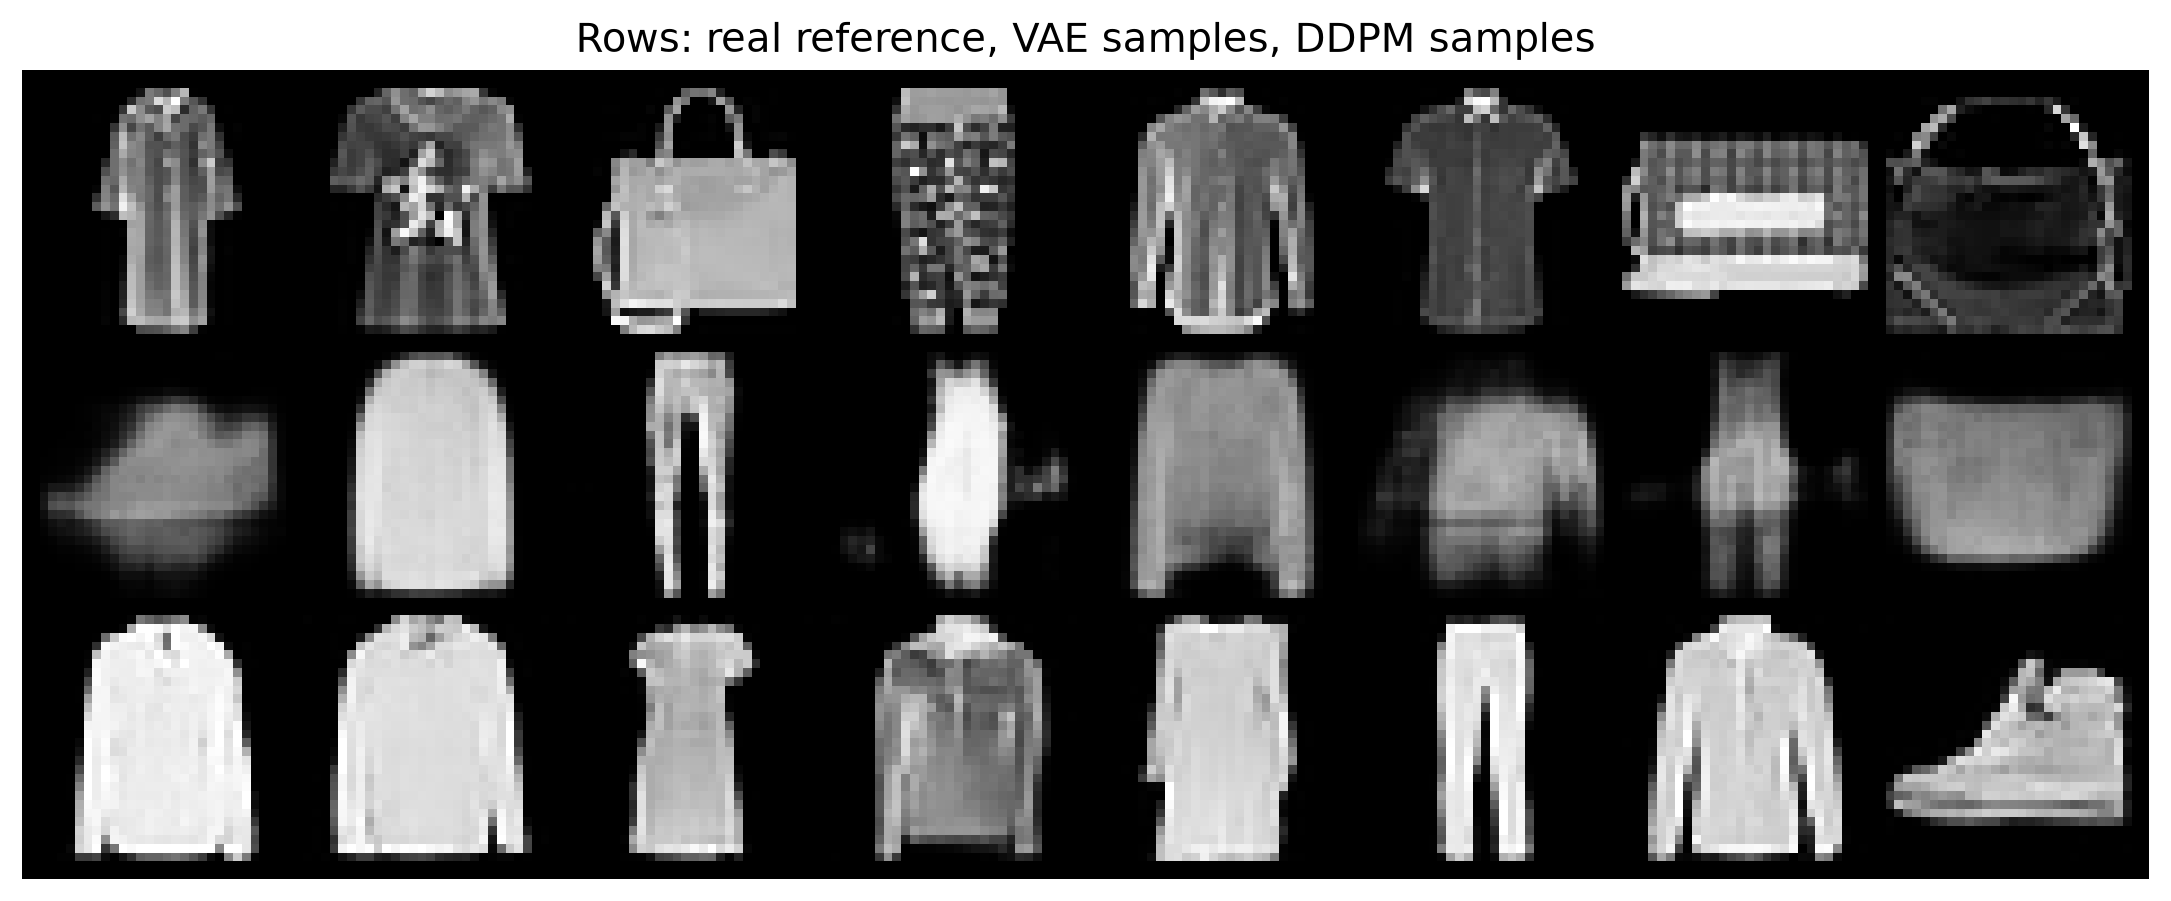
\includegraphics[width=0.96\linewidth]{figures/main/real_vae_ddpm_comparison.png}
  \caption{Real Fashion-MNIST images and generated samples from the VAE and DDPM.}
  \label{fig:samples}
\end{figure}

The models also show different generation behavior. Figure~\ref{fig:generation} shows a VAE interpolation between the latent means of two test images and a DDPM denoising trajectory. The VAE changes the decoded output smoothly as the latent representation is interpolated, while the DDPM gradually forms a recognizable image from random noise over repeated reverse steps.

\begin{figure}[t]
\centering
\begin{minipage}{0.48\linewidth}
\centering
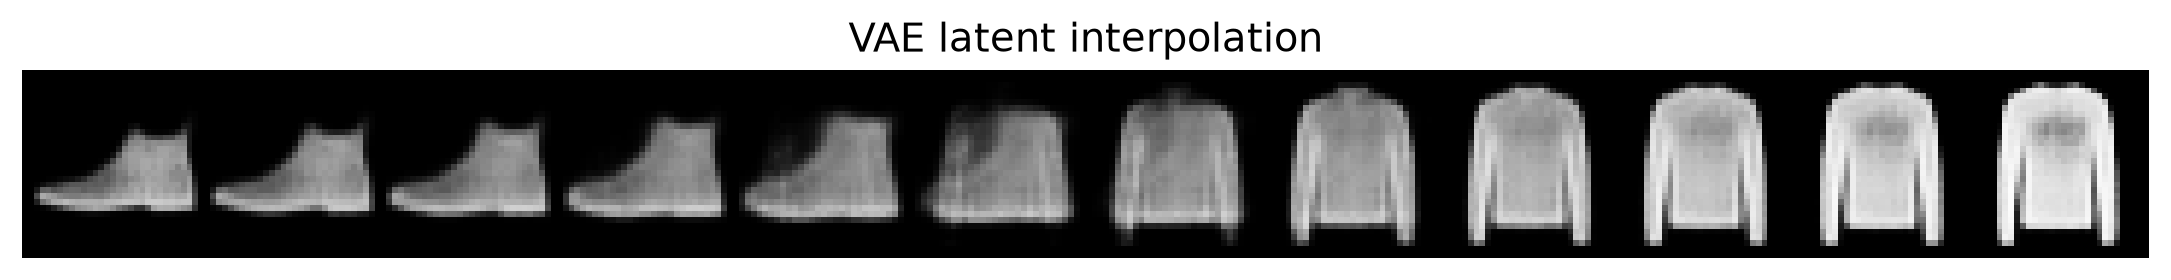
\includegraphics[width=\linewidth]{figures/main/vae_latent_interpolation.png}
\small (a) VAE latent interpolation
\end{minipage}
\hfill
\begin{minipage}{0.48\linewidth}
\centering
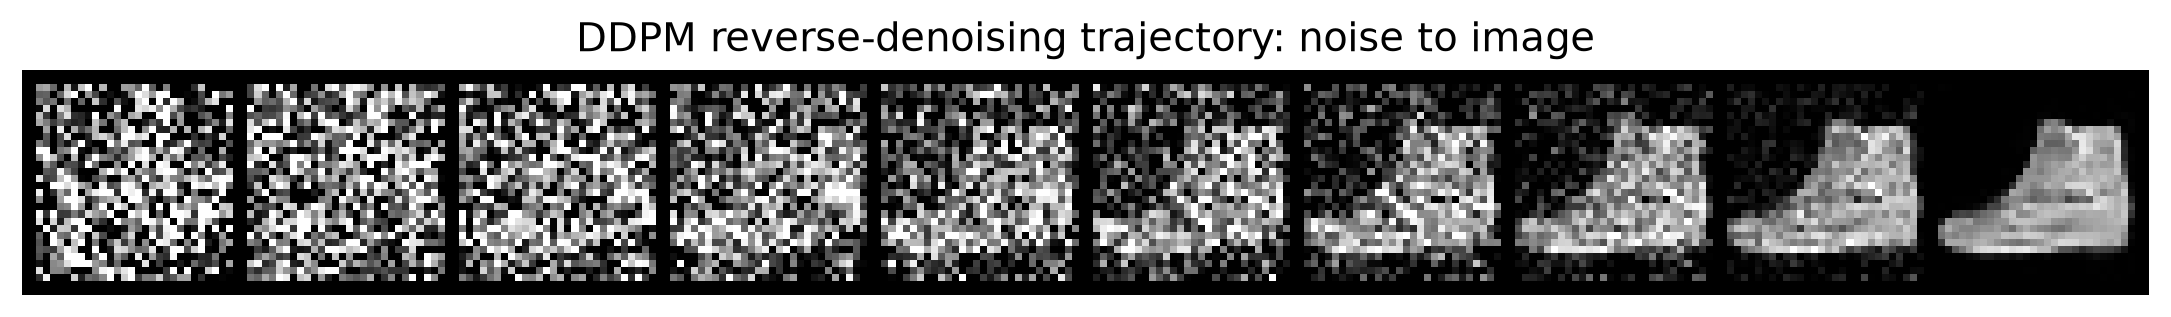
\includegraphics[width=\linewidth]{figures/main/ddpm_denoising_trajectory.png}
\small (b) DDPM denoising trajectory
\end{minipage}
\caption{Different generation structures of the two models.}
\label{fig:generation}
\end{figure}

\subsection{Quantitative Results}
Table~\ref{tab:results} gives the main comparison across ten independent runs, each using 5,000 generated samples per model. The DDPM achieves a much lower mean classifier-feature FID ($11.14 \pm 5.79$ versus $43.32 \pm 4.51$) and KID ($0.530 \pm 0.342$ versus $1.807 \pm 0.268$), indicating that its generated feature distribution is consistently closer to the real reference set. The classifier also assigns higher average confidence to DDPM samples, and $67.11\% \pm 2.93\%$ of DDPM samples reach at least 0.8 confidence compared with $43.37\% \pm 1.59\%$ for the VAE.

\begin{table}[t]
\caption{Main quantitative comparison. Higher is better for confidence, recognizability, and entropy; lower is better for FID, KID, and time.}
\label{tab:results}
\centering
\small
\begin{tabular}{lrr}
\toprule
Metric & VAE & DDPM \\
\midrule
Classifier-feature FID $\downarrow$ & $43.32 \pm 4.51$ & $\mathbf{11.14 \pm 5.79}$ \\
Classifier-feature KID $\downarrow$ & $1.807 \pm 0.268$ & $\mathbf{0.530 \pm 0.342}$ \\
Mean classifier confidence $\uparrow$ & $0.717 \pm 0.009$ & $\mathbf{0.841 \pm 0.014}$ \\
Confidence $\geq 0.8$ $\uparrow$ & $43.37\% \pm 1.59\%$ & $\mathbf{67.11\% \pm 2.93\%}$ \\
Class coverage & $10/10$ & $10/10$ \\
Normalized class entropy $\uparrow$ & $0.941 \pm 0.013$ & $\mathbf{0.971 \pm 0.028}$ \\
Training time $\downarrow$ & $\mathbf{0.411 \pm 0.020}$ min & $4.811 \pm 0.059$ min \\
Sampling time $\downarrow$ & $\mathbf{0.00784 \pm 0.00062}$ ms/img & $8.173 \pm 0.110$ ms/img \\
\bottomrule
\end{tabular}
\end{table}

Both models cover all 10 predicted Fashion-MNIST classes in every run, but their distributions are not equally balanced. The VAE reaches normalized class entropy $0.941 \pm 0.013$, while the DDPM reaches $0.971 \pm 0.028$. The higher DDPM mean indicates a distribution closer to uniform, although its larger standard deviation also shows greater run-to-run variation in balance. Both training procedures complete without non-finite losses across all ten seeds. The final VAE negative ELBO is $236.387 \pm 0.095$, while the DDPM noise-prediction MSE is $0.07036 \pm 0.00038$. These losses are not directly comparable because the models optimize different objectives.

\begin{figure}[t]
  \centering
  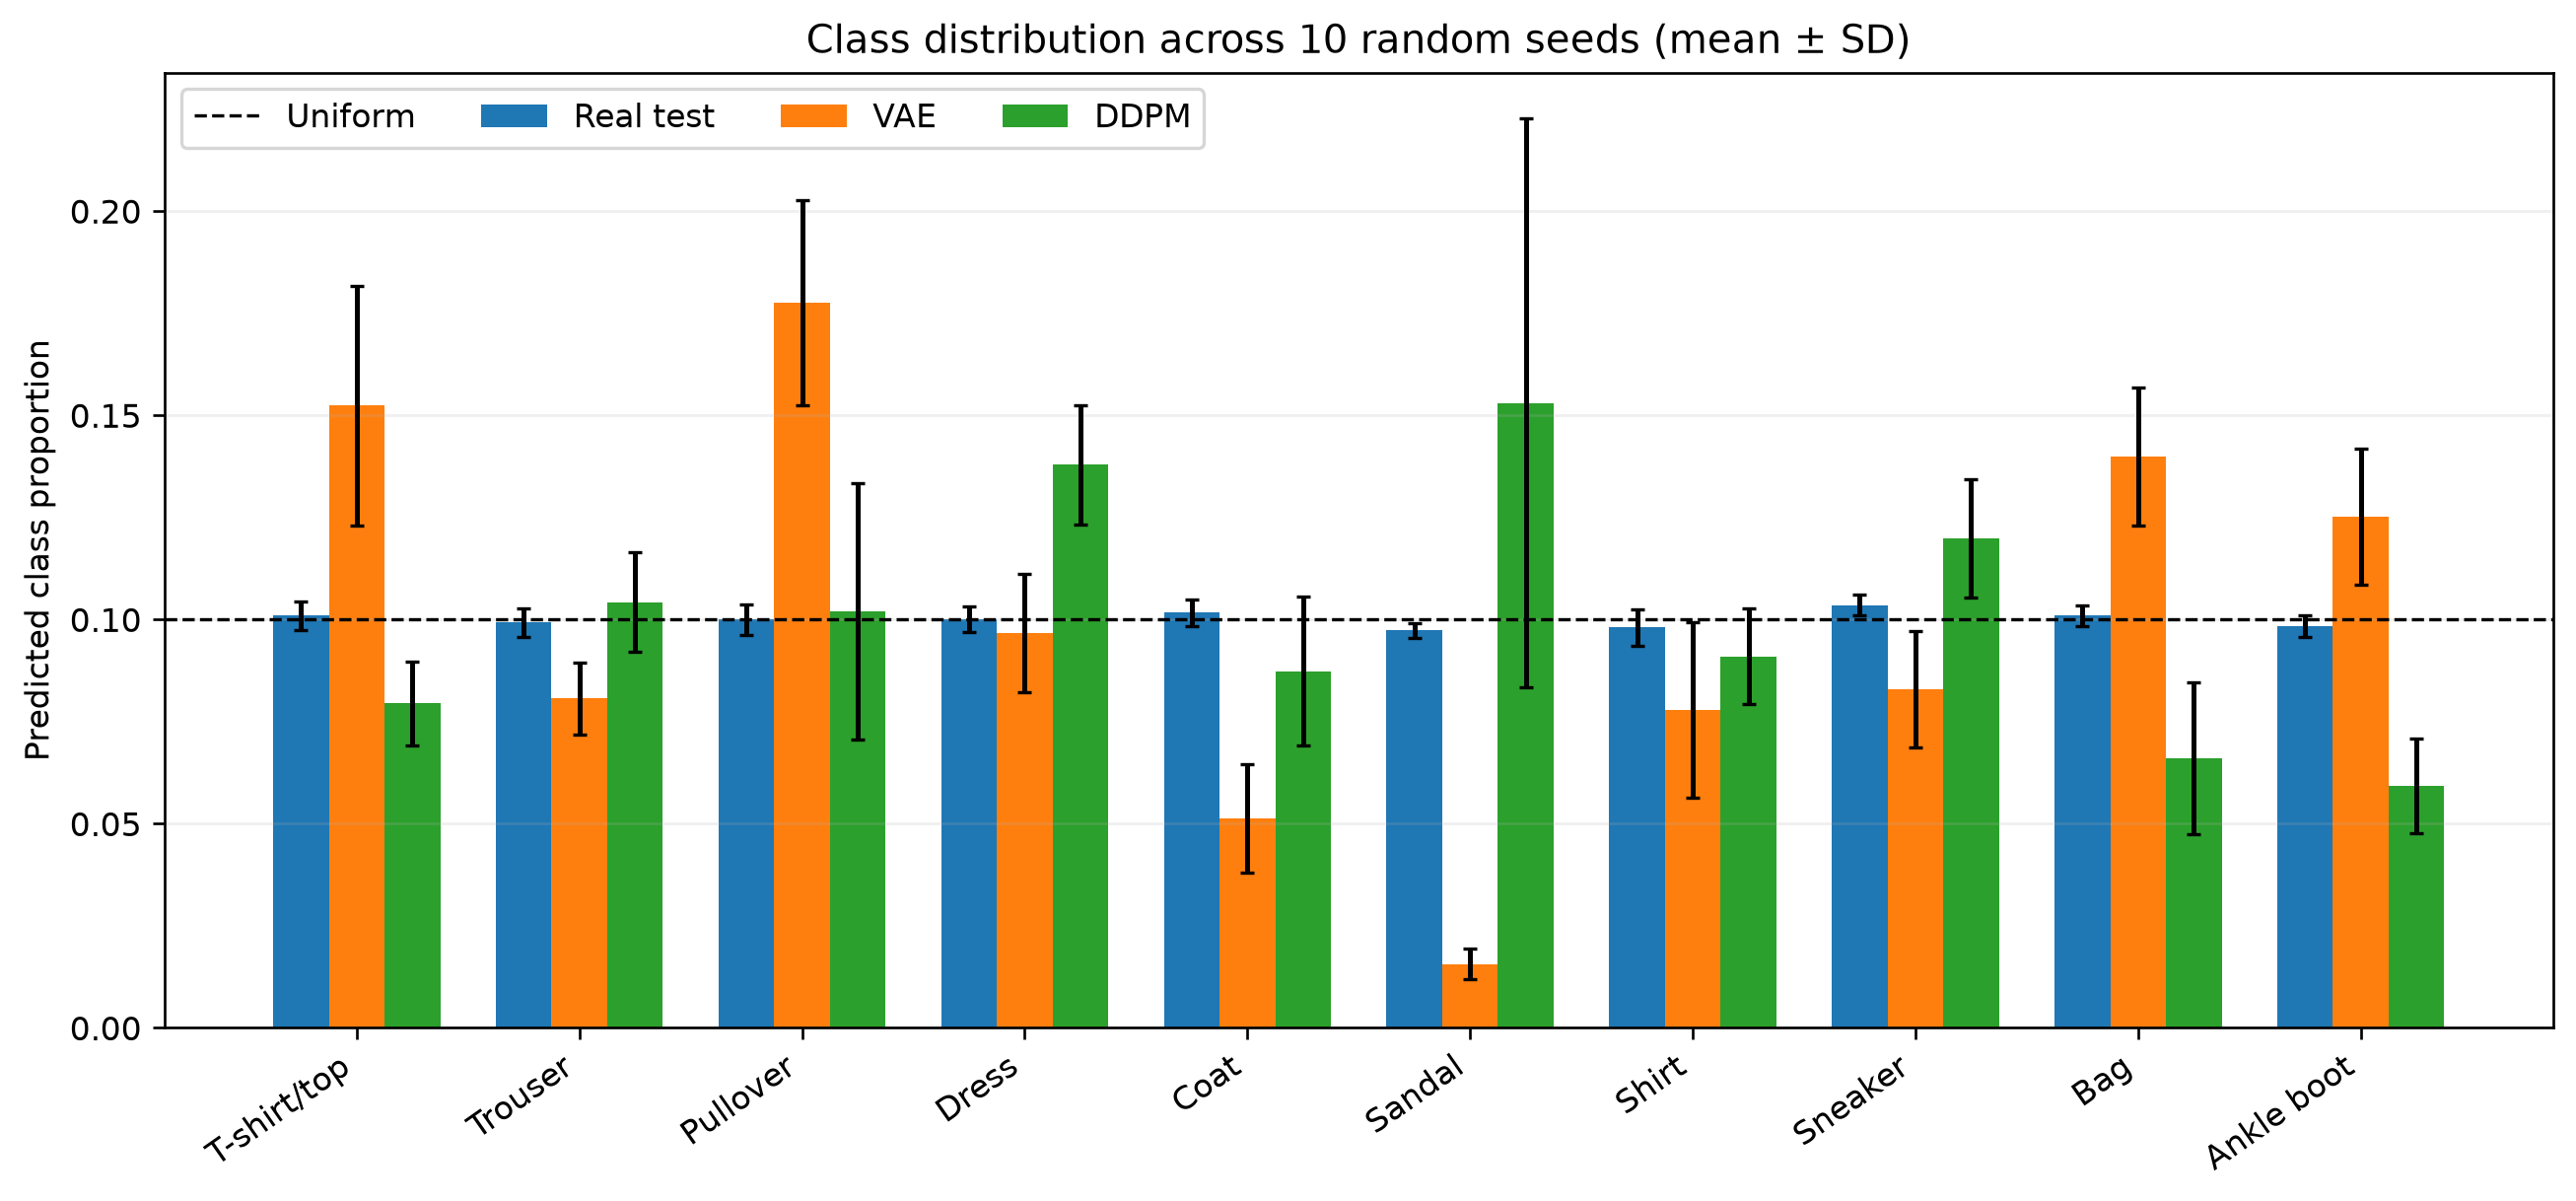
\includegraphics[width=0.88\linewidth]{figures/multiseed/class_distribution_multiseed.png}
  \caption{Predicted class distribution across ten seeds, with 5,000 generated samples per model per seed. Bars show means and error bars show sample standard deviations. The dashed line denotes the uniform proportion of 0.1.}
  \label{fig:class_distribution}
\end{figure}

The largest cost difference appears during sampling. VAE sampling takes $0.00784 \pm 0.00062$ ms per image in the recorded batched experiments, whereas DDPM sampling takes $8.173 \pm 0.110$ ms per image. This is expected from the implementations: the VAE generates an image with a single decoder pass, while the DDPM performs 100 sequential denoising steps. Mean training time also increases from $0.411 \pm 0.020$ minutes for the VAE to $4.811 \pm 0.059$ minutes for the DDPM. Peak GPU allocation is constant at 558 MB for the VAE and 6275 MB for the DDPM under the fixed configuration. The feature-space memorization-screen rate averages $0.31\% \pm 0.40\%$ for the VAE and $1.17\% \pm 1.12\%$ for the DDPM under a strict threshold defined by the 1st percentile of real-image nearest-neighbor distances. We therefore do not observe strong evidence of direct training-set memorization, although this screen is not a proof that memorization is absent.

\begin{figure}[t]
\centering
\begin{minipage}{0.48\linewidth}
\centering
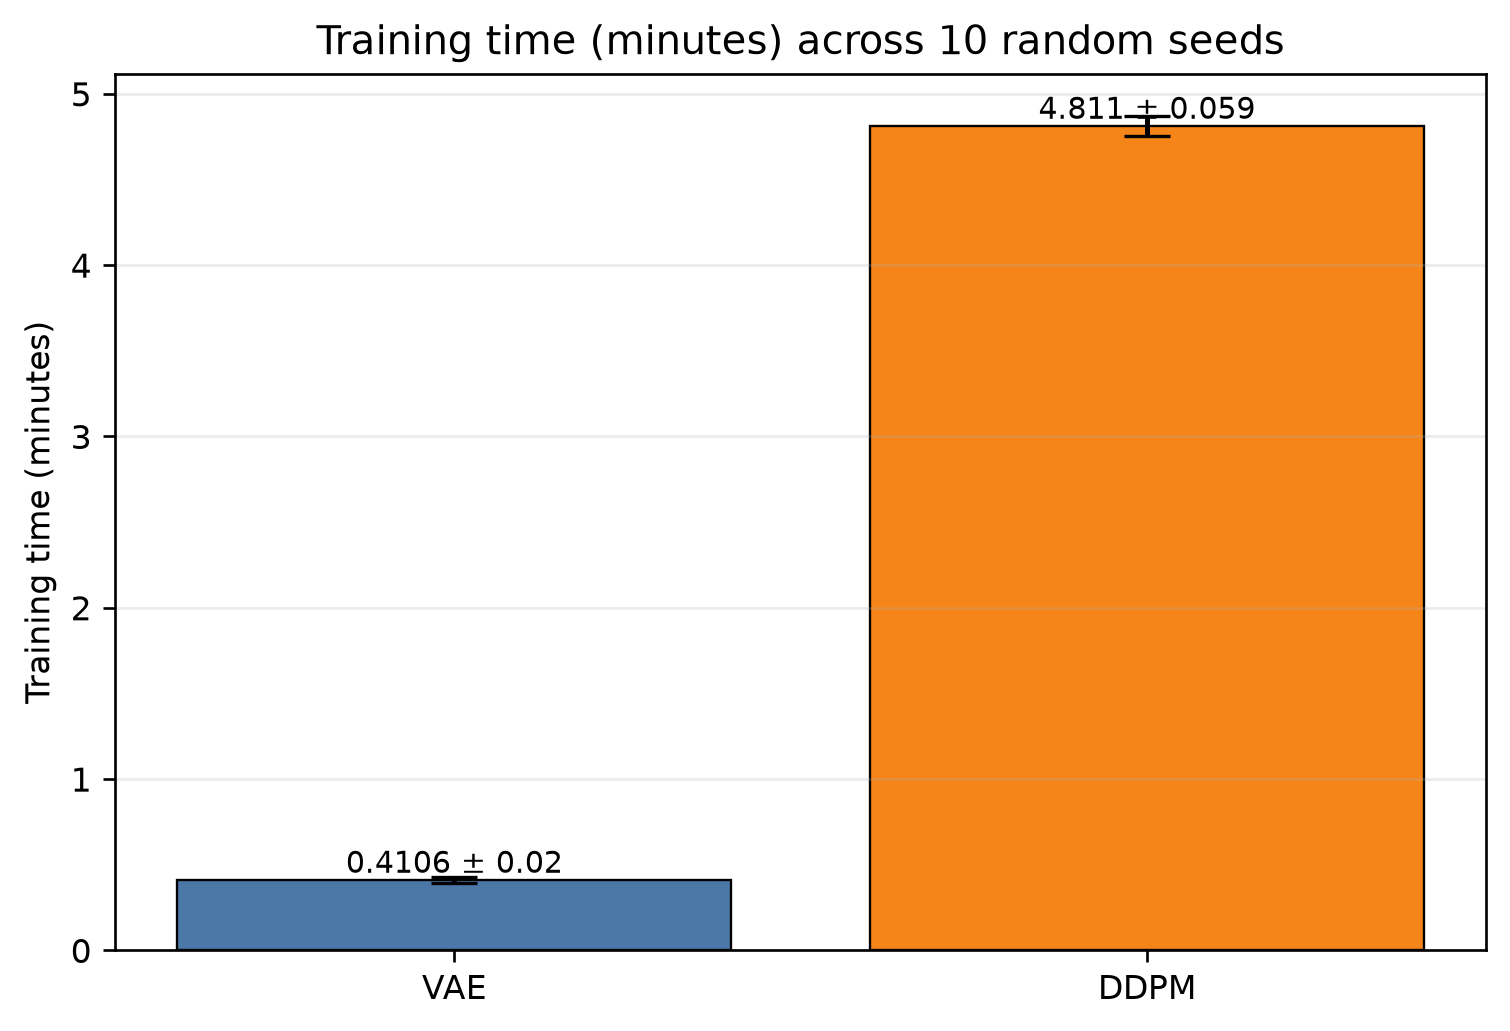
\includegraphics[width=\linewidth]{figures/multiseed/training_minutes_multiseed.png}
\small (a) Measured training time
\end{minipage}
\hfill
\begin{minipage}{0.48\linewidth}
\centering
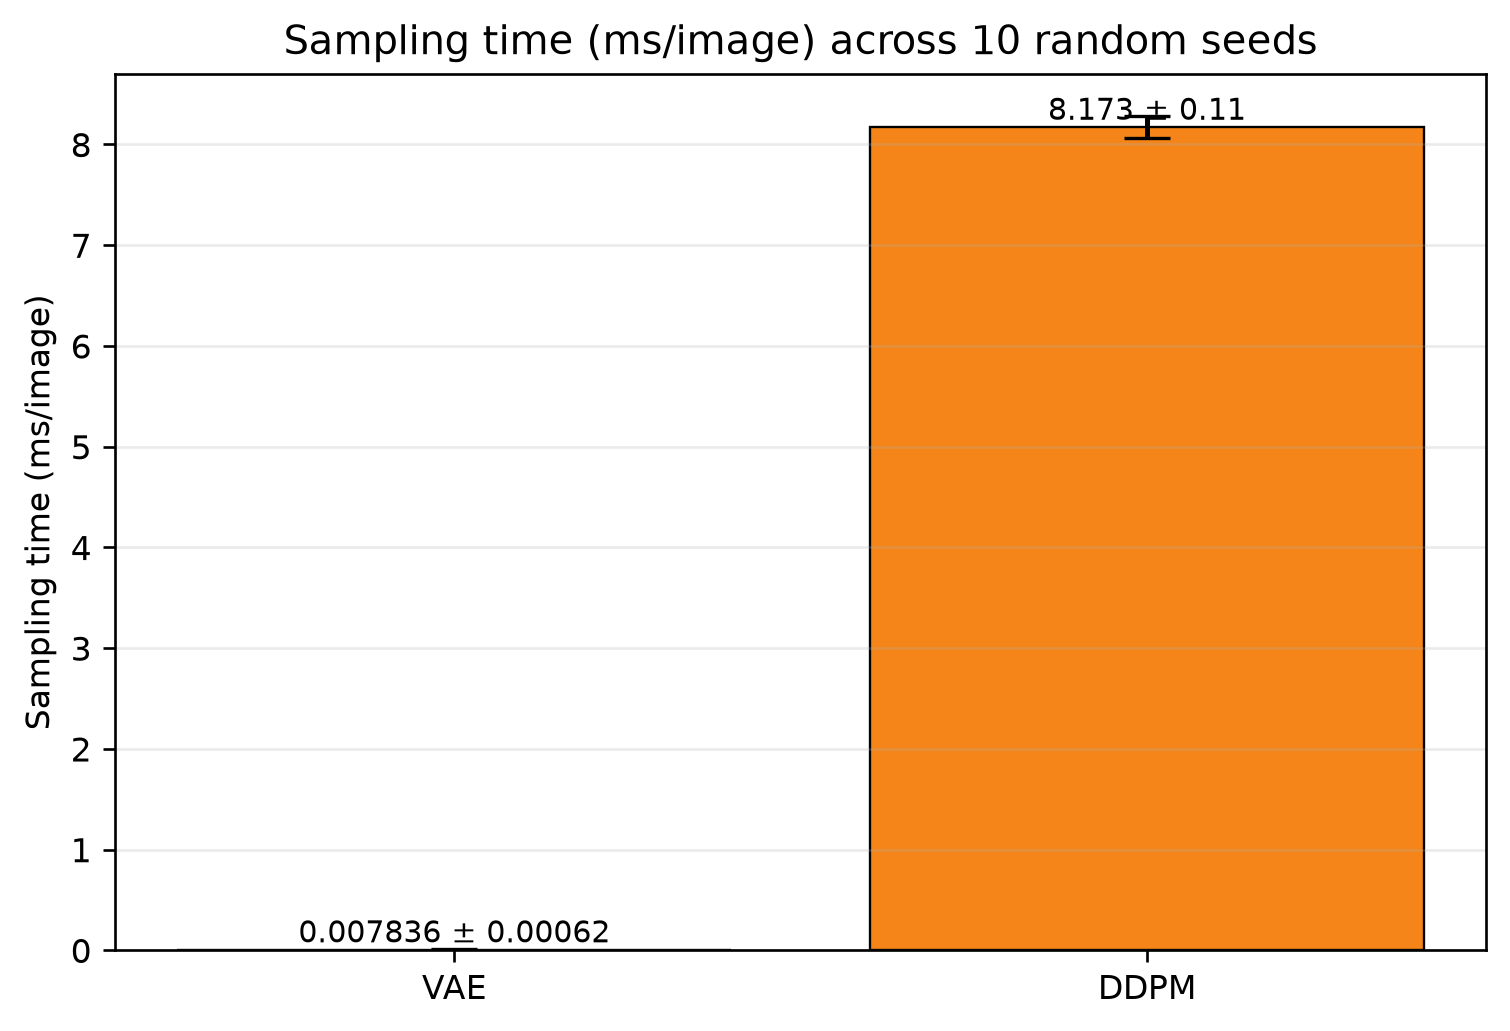
\includegraphics[width=\linewidth]{figures/multiseed/sampling_ms_per_image_multiseed.png}
\small (b) Batched sampling time per image
\end{minipage}
\caption{Computational cost comparison on the same RTX 5070 Ti system. The measurements characterize this implementation and batch configuration rather than hardware-independent algorithmic constants.}
\label{fig:compute_cost}
\end{figure}

\section{Discussion}
The results show that the DDPM performs better on most of the measured generation-quality indicators in our implementation. Its sample grid is visually sharper, its classifier-feature FID and KID are substantially lower, and generated images receive higher classifier confidence. The class-distribution results also show why class coverage alone is not enough to describe diversity. Although both models generated all 10 predicted classes, the VAE distribution is noticeably more concentrated in several classes, while the DDPM is more balanced.

The main advantage of the VAE is efficiency. It uses fewer trainable parameters and requires much less measured training time and GPU memory. Its direct latent-space sampling is also over three orders of magnitude faster per image than the 100-step DDPM sampling procedure in this experiment. The two models therefore show a clear quality--efficiency trade-off rather than one model being better in every aspect.

The magnitude of the gaps helps distinguish structural costs from implementation details. The DDPM has approximately 3.1 times as many trainable parameters, but mean training is about 11.7 times slower and sampling about 1,043 times slower per image. Parameter count alone therefore cannot explain the sampling gap; the dominant factor is the sequence of 100 reverse evaluations. Conversely, the DDPM's much lower classifier-feature FID and more uniform predicted class distribution across ten seeds suggest that iterative refinement is doing more than merely increasing capacity. A parameter-matched ablation would be required to isolate those two effects rigorously.

There are several limitations to this comparison. Ten seeds quantify run-to-run variation, but we do not perform formal paired hypothesis tests or report confidence intervals. The DDPM is also larger than the VAE (5.22M versus 1.70M trainable parameters), so the experiment is a comparison of our two implemented systems rather than a parameter-matched architecture study. Finally, FID, KID, recognizability, and class-distribution measurements depend on the Fashion-MNIST evaluators. Their mean $91.37\% \pm 0.20\%$ test accuracy makes them useful for evaluation, but these classifier-based metrics should still be interpreted together with visual samples.

Timing is another external-validity limitation. The reported values use one RTX 5070 Ti, mixed precision, large batches, and implementation-specific optimizations. They are useful for within-system comparison but should not be treated as universal latency estimates. The nearest-neighbor analysis is also a screen rather than a proof: it uses a finite reference subset and a learned feature space, so exact or perceptual memorization outside that representation may remain undetected. Finally, class entropy measures balance across predicted labels, not diversity within each label. Repeated seeds, per-class diversity analysis, human evaluation, and precision--recall style distribution metrics would strengthen the conclusions.

\section{Conclusions}
We implemented and evaluated a convolutional VAE and a DDPM on Fashion-MNIST under a shared experimental pipeline. Both models generated recognizable samples, but the DDPM produced sharper images, better classifier-feature distribution scores, and a more balanced predicted class distribution. The VAE was much more computationally efficient, especially during sampling. Future work could repeat the experiment across multiple random seeds and compare models with more closely matched parameter counts or fewer DDPM sampling steps.

\section*{References}
\small
[1] D. P. Kingma and M. Welling. ``Auto-Encoding Variational Bayes.'' arXiv:1312.6114, 2013.

[2] J. Ho, A. Jain, and P. Abbeel. ``Denoising Diffusion Probabilistic Models.'' arXiv:2006.11239, 2020.

[3] H. Xiao, K. Rasul, and R. Vollgraf. ``Fashion-MNIST: A Novel Image Dataset for Benchmarking Machine Learning Algorithms.'' arXiv:1708.07747, 2017.

[4] M. Heusel, H. Ramsauer, T. Unterthiner, B. Nessler, and S. Hochreiter. ``GANs Trained by a Two Time-Scale Update Rule Converge to a Local Nash Equilibrium.'' Advances in Neural Information Processing Systems, 2017.

[5] M. Bi\'nkowski, D. J. Sutherland, M. Arbel, and A. Gretton. ``Demystifying MMD GANs.'' arXiv:1801.01401, 2018.

\section*{Appendix}
The following repository outputs are included as supplementary evidence for the main comparison.

\begin{figure}[h]
  \centering
  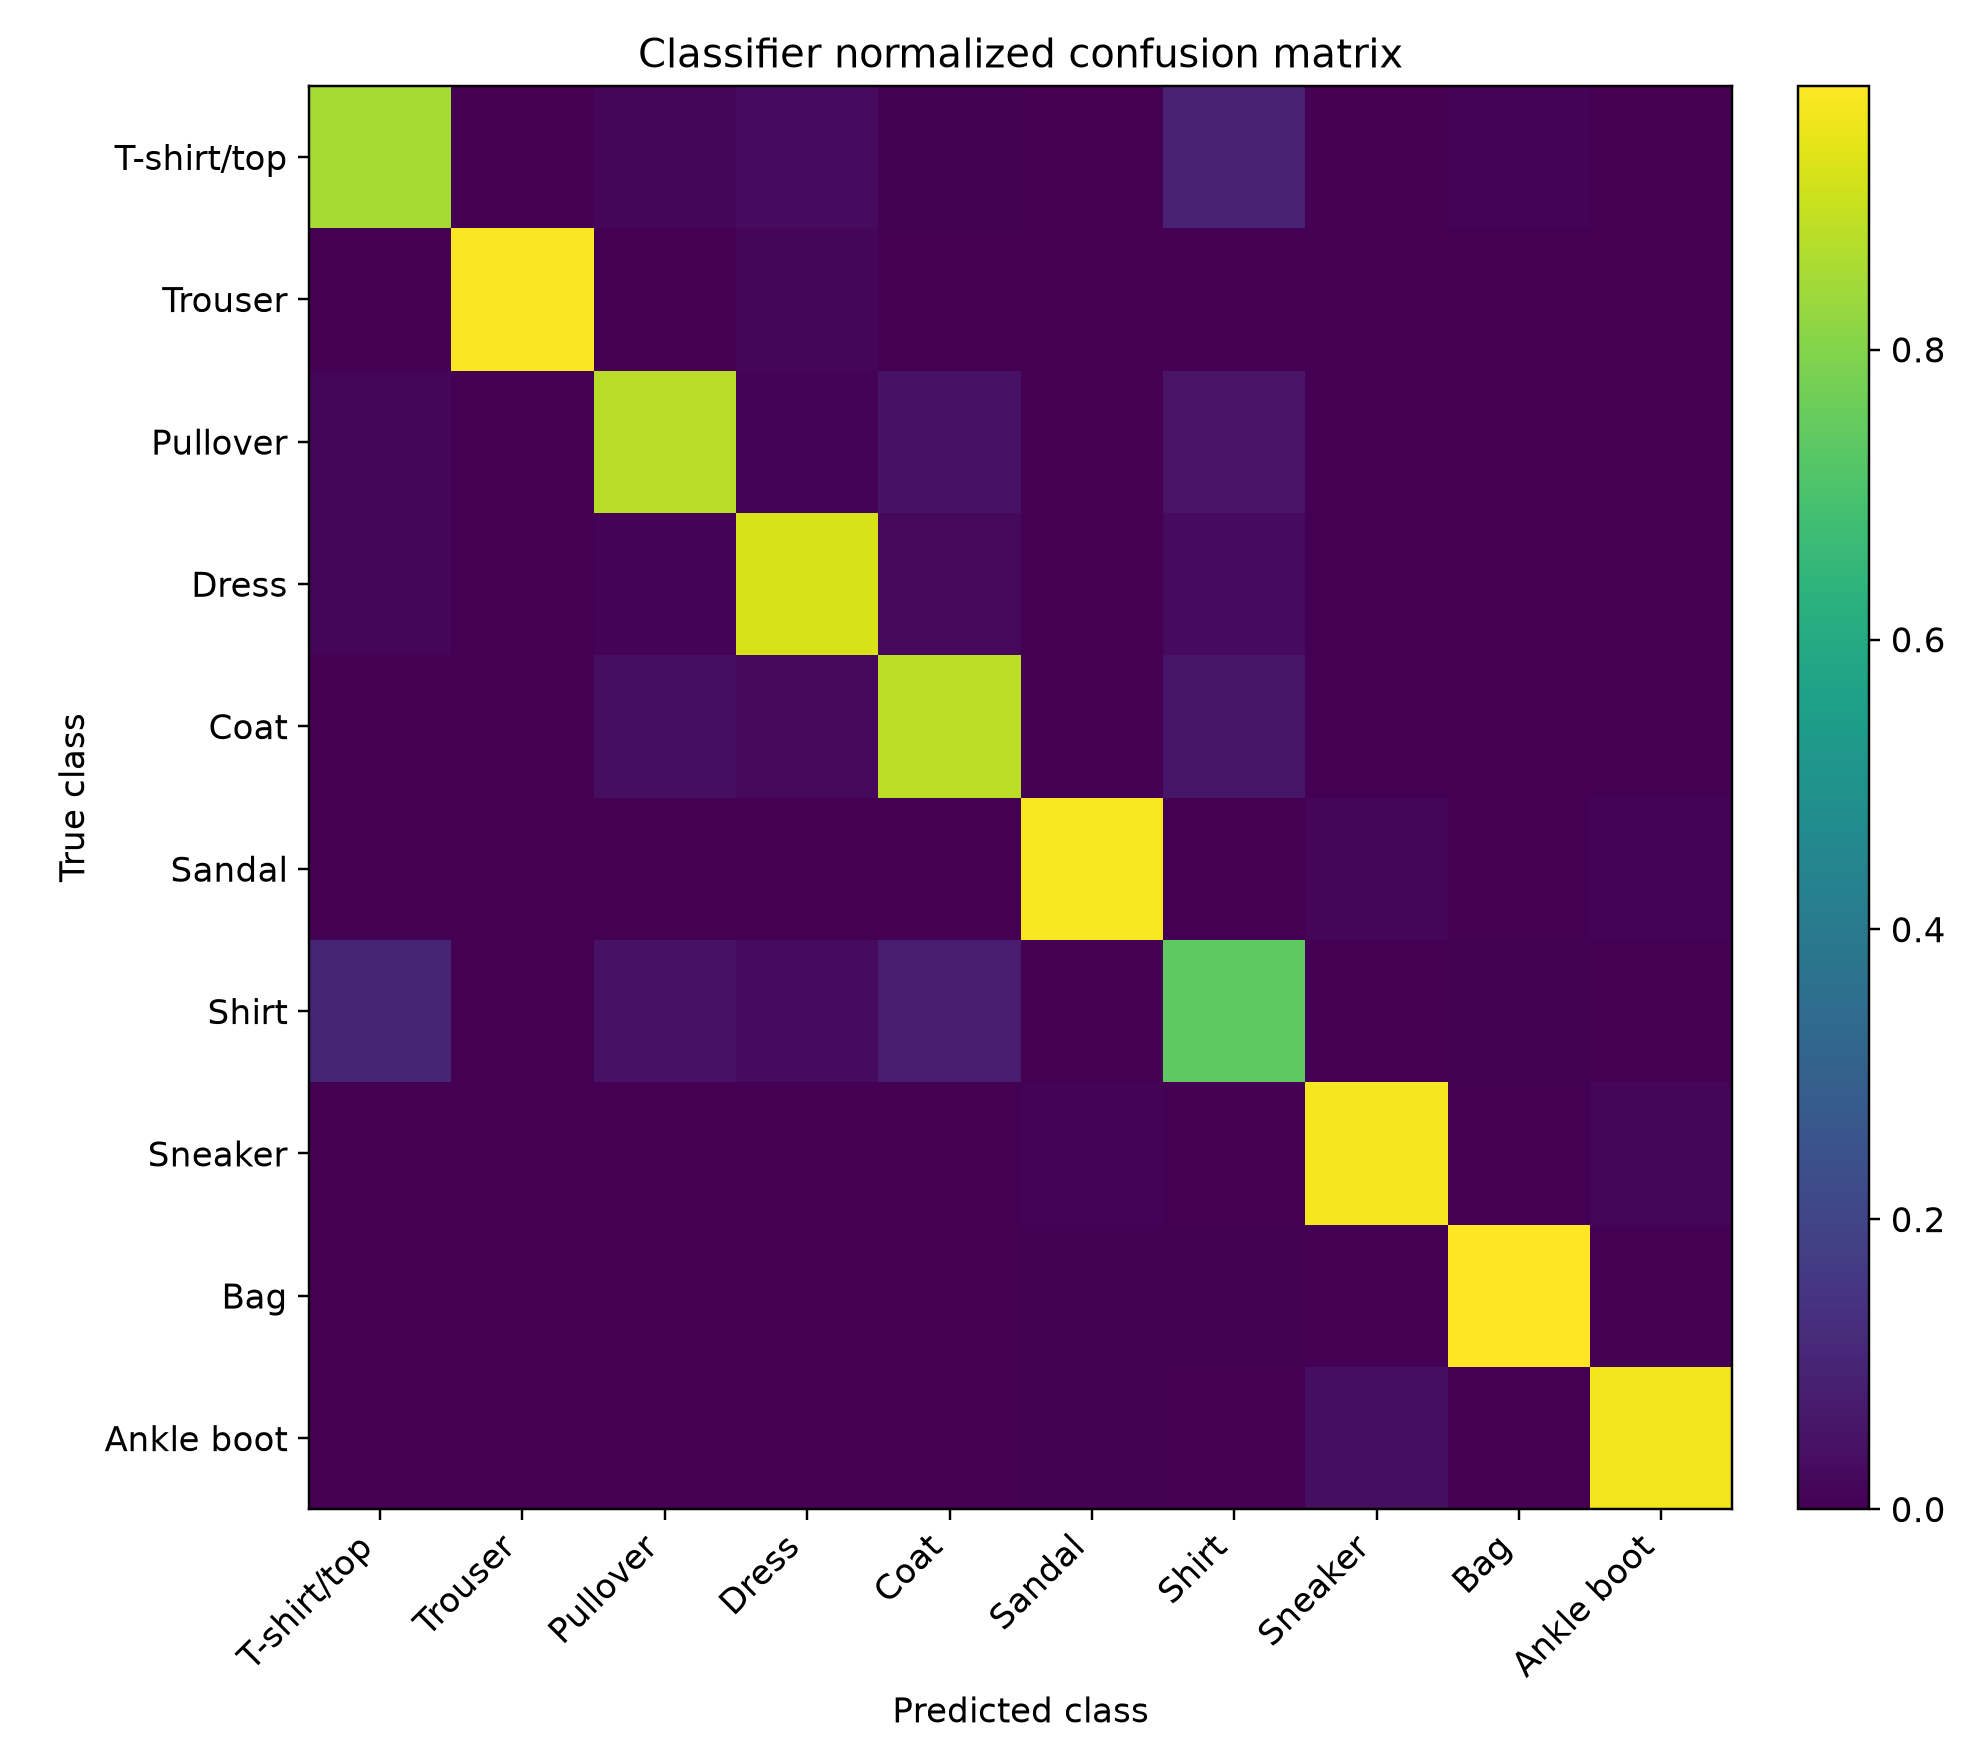
\includegraphics[width=0.92\linewidth]{figures/appendix/classifier_confusion_matrix.png}
  \caption{Confusion matrix for one representative Fashion-MNIST evaluation classifier. Across ten runs, evaluator accuracy is $91.37\% \pm 0.20\%$, supporting its use while also showing that classifier-derived metrics are imperfect.}
\end{figure}

\begin{figure}[h]
\centering
\begin{minipage}{0.48\linewidth}
\centering
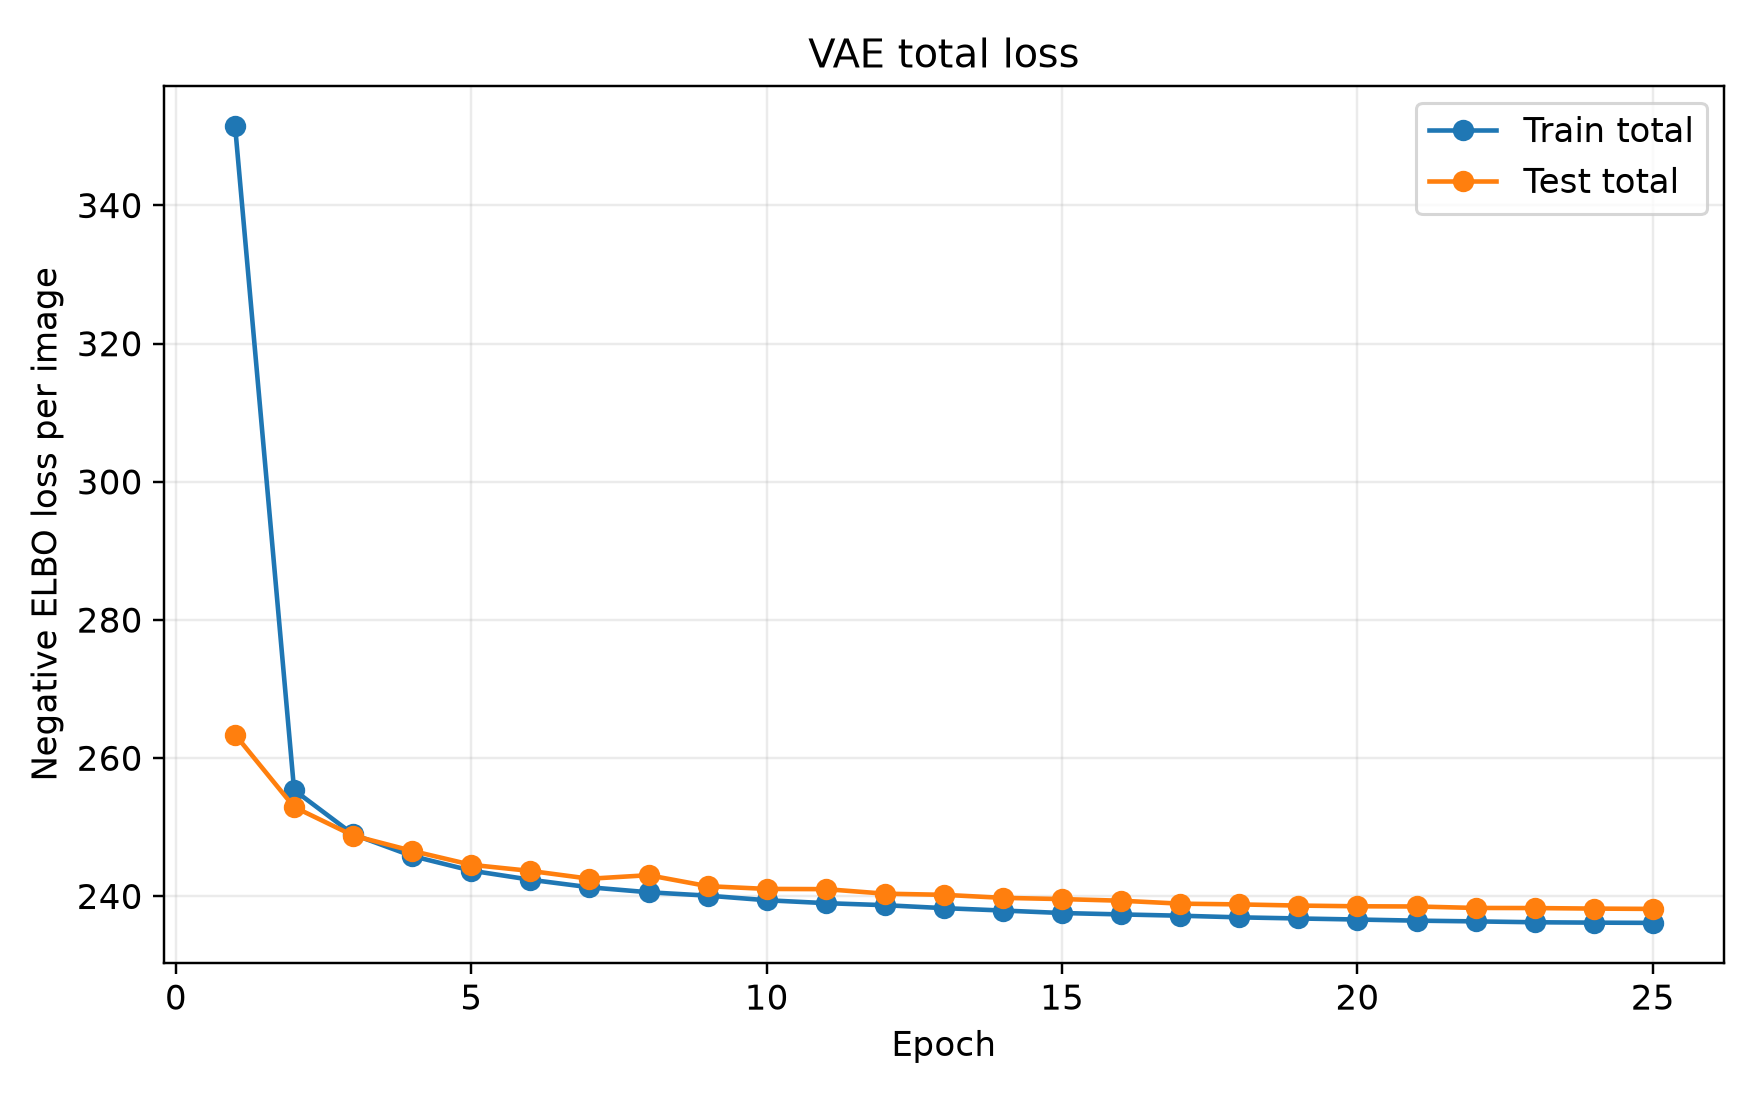
\includegraphics[width=\linewidth]{figures/appendix/vae_total_loss.png}
\small (a) VAE negative ELBO
\end{minipage}
\hfill
\begin{minipage}{0.48\linewidth}
\centering
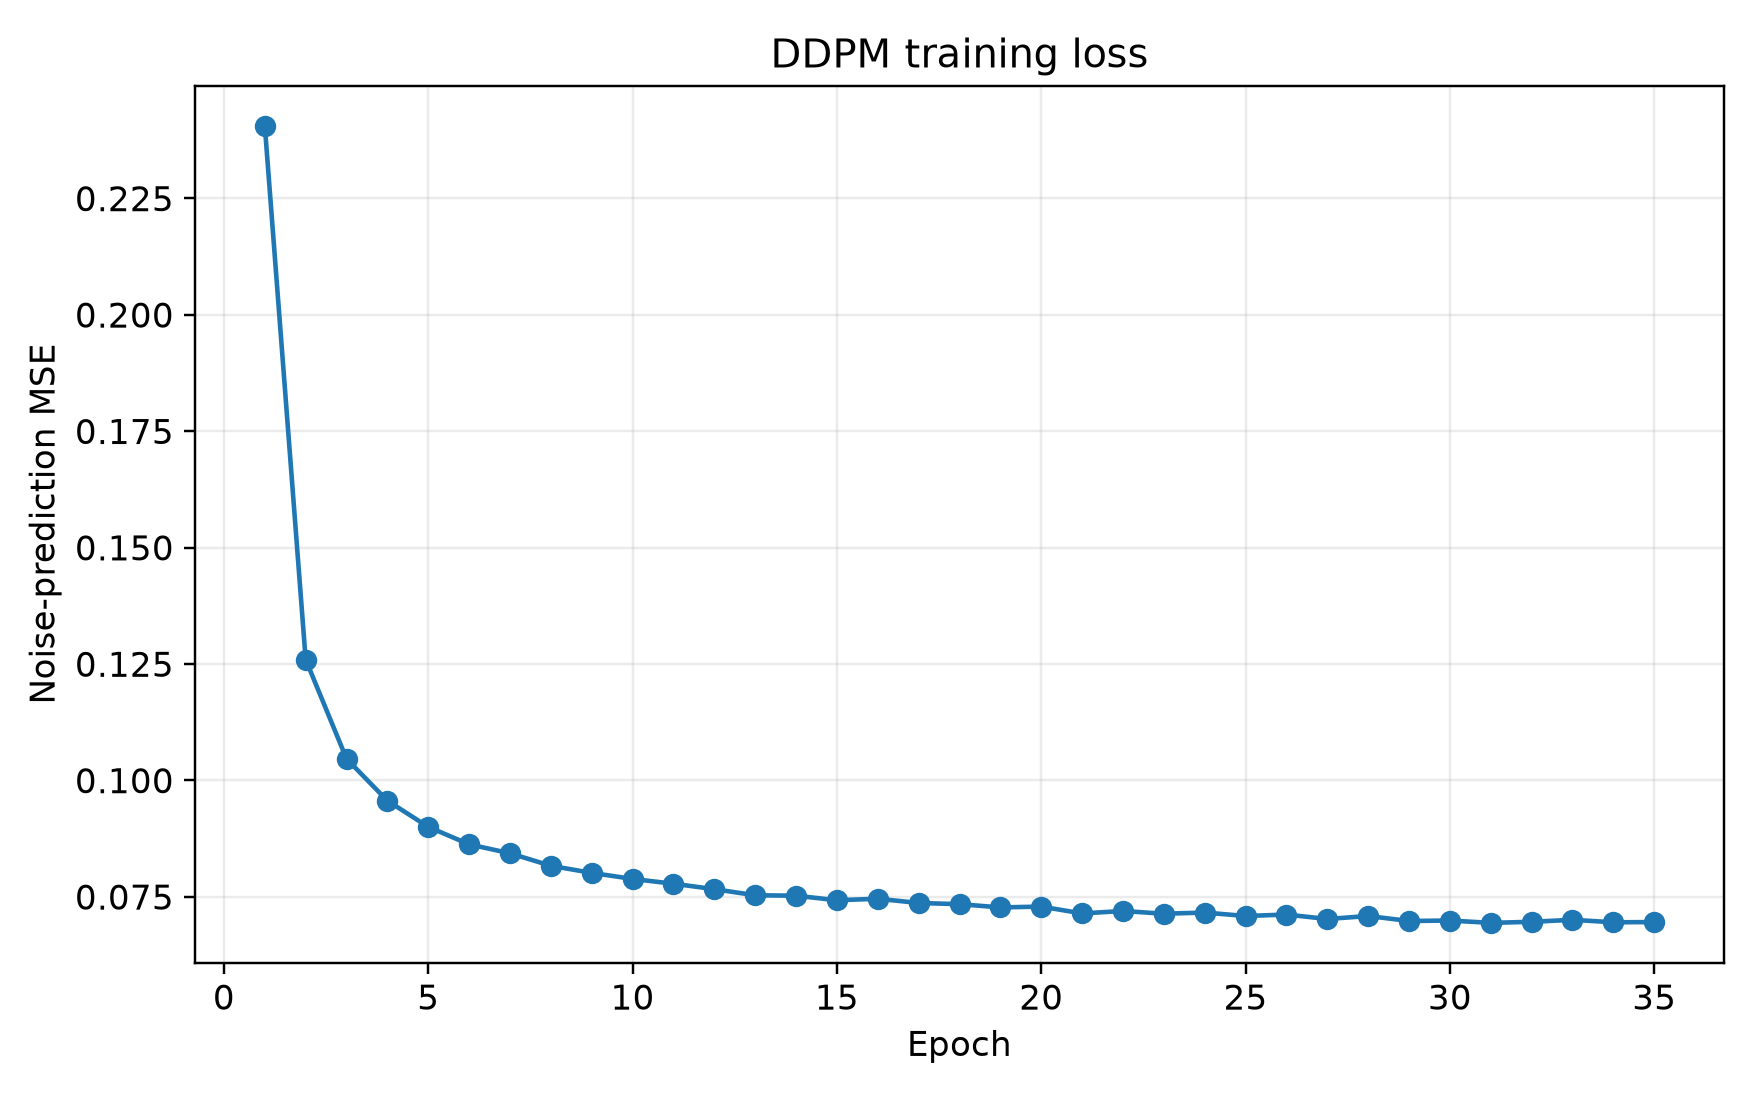
\includegraphics[width=\linewidth]{figures/appendix/ddpm_noise_prediction_loss.png}
\small (b) DDPM noise-prediction MSE
\end{minipage}
\caption{Training curves for the two models. The absolute loss values are not directly comparable because the objectives are different.}
\end{figure}

\begin{figure}[h]
\centering
\begin{minipage}{0.48\linewidth}
\centering
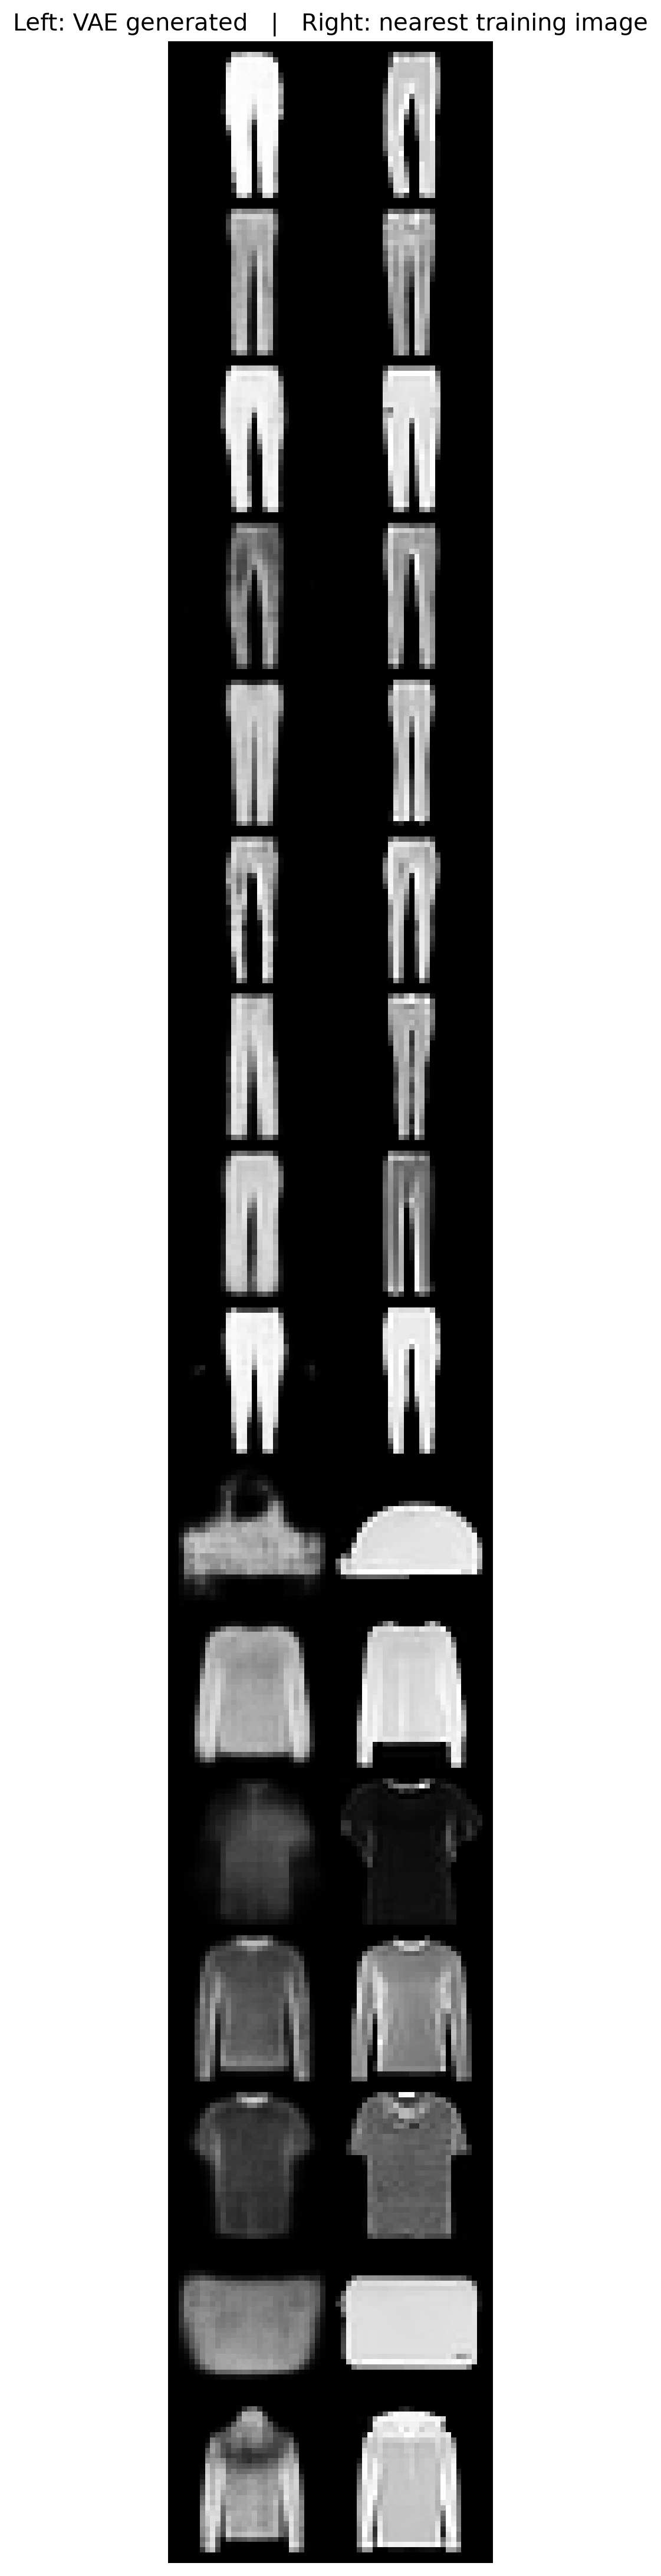
\includegraphics[width=\linewidth]{figures/appendix/vae_nearest_neighbors.png}
\small (a) VAE nearest neighbors
\end{minipage}
\hfill
\begin{minipage}{0.48\linewidth}
\centering
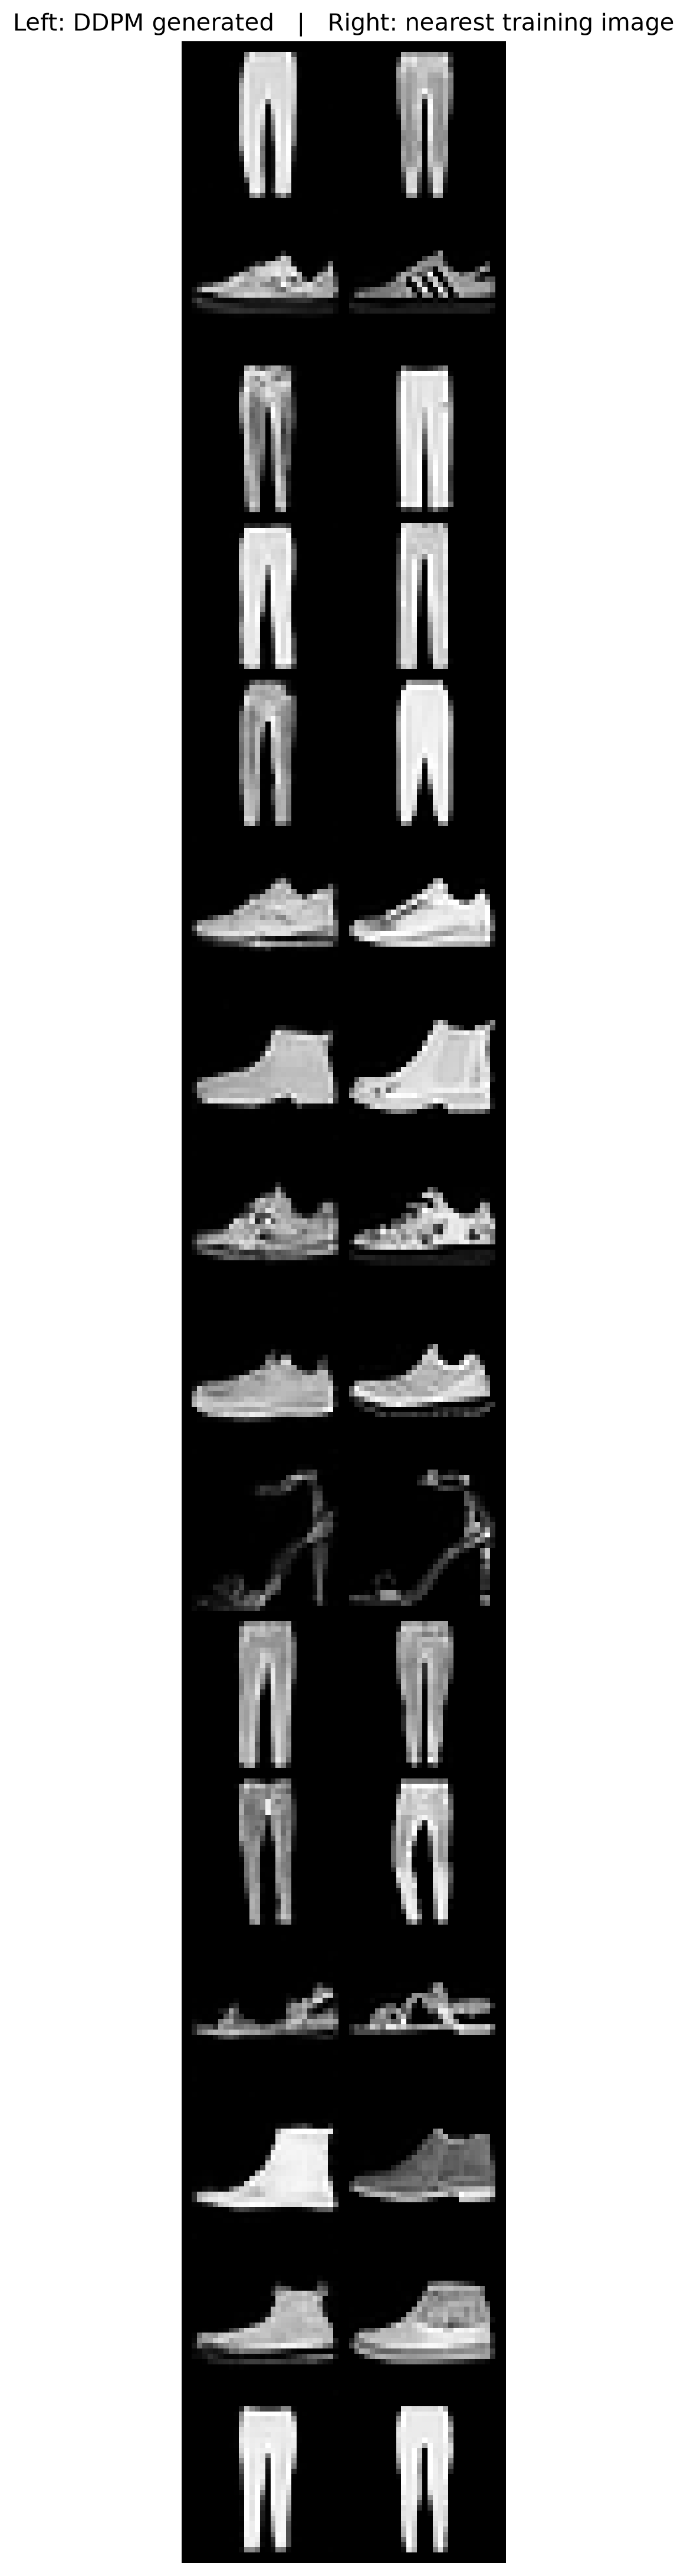
\includegraphics[width=\linewidth]{figures/appendix/ddpm_nearest_neighbors.png}
\small (b) DDPM nearest neighbors
\end{minipage}
\caption{Feature-space nearest-neighbor examples used as a limited memorization screen. Visual similarity is expected for simple Fashion-MNIST classes and does not by itself establish copying.}
\end{figure}

\end{document}
